\documentclass{standalone}
\usepackage[utf8]{inputenc}
\usepackage{newtxtext}
\usepackage{newtxmath}
\usepackage[italic]{hepnicenames}
\makeatletter\def\@shiftlen@anti@gen@bar{0mu}\makeatother
\usepackage[svgnames]{xcolor}
\usepackage{tikz-feynhand}


\begin{document}
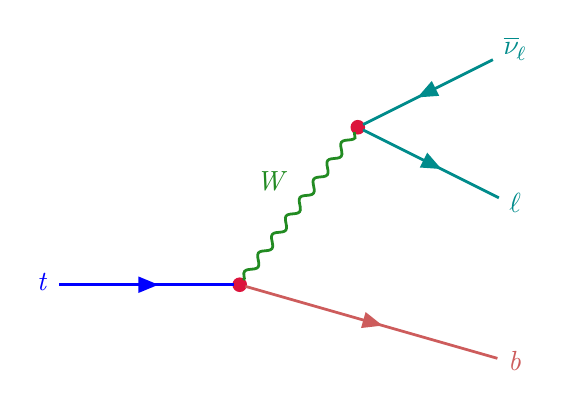
\begin{tikzpicture}
  \setlength{\feynhandlinesize}{1.0pt}
  \tikzfeynhandset{every dot={/tikz/color=Crimson},}
  \begin{feynhand}
    \vertex [particle, Blue] (t) at (-3.0, 1.0) {\Ptop};
    \vertex [particle, IndianRed] (b) at (3.0, 0.0) {\Pbottom};
    \vertex [particle, DarkCyan] (l) at (3.0, 2.0) {\color{DarkCyan}\Plepton};
    \vertex [particle, DarkCyan] (nu) at (3.0, 4.0) {\color{DarkCyan}\APnulepton};
    \vertex [dot, Crimson] (tb) at (-0.5, 1.0) {};
    \vertex [dot, Crimson] (Wlnu) at (1.0, 3.0) {};
    \propagator [fermion, Blue] (t) to (tb);
    \propagator [fermion, IndianRed] (tb) to (b);
    \propagator [boson, ForestGreen] (tb) to [edge label=\PW, color=ForestGreen] (Wlnu);
    \propagator [fermion, DarkCyan] (Wlnu) to (l);
    \propagator [fermion, DarkCyan] (nu) to (Wlnu);
  \end{feynhand}
\end{tikzpicture}
\end{document}
